\documentclass{article}


% if you need to pass options to natbib, use, e.g.:
%     \PassOptionsToPackage{numbers, compress}{natbib}
% before loading neurips_2022


% ready for submission
% \usepackage{neurips_2022}


% to compile a preprint version, e.g., for submission to arXiv, add add the
% [preprint] option:
\usepackage[preprint]{neurips_2022}


% to compile a camera-ready version, add the [final] option, e.g.:
% \usepackage[final]{neurips_2022}


% to avoid loading the natbib package, add option nonatbib:
%    \usepackage[nonatbib]{neurips_2022}


\usepackage[utf8]{inputenc} % allow utf-8 input
\usepackage[T1]{fontenc}    % use 8-bit T1 fonts
\usepackage{hyperref}       % hyperlinks
\usepackage{url}            % simple URL typesetting
\usepackage{booktabs}       % professional-quality tables
\usepackage{amsfonts}       % blackboard math symbols
\usepackage{nicefrac}       % compact symbols for 1/2, etc.
\usepackage{microtype}      % microtypography
\usepackage{xcolor}         % colors

% my personal packages
\usepackage{tablefootnote}
\usepackage{graphicx}
\bibliographystyle{abbrvnat}

\title{Getting on with Life(Steps): a simulation based on daily life decisions}


% The \author macro works with any number of authors. There are two commands
% used to separate the names and addresses of multiple authors: \And and \AND.
%
% Using \And between authors leaves it to LaTeX to determine where to break the
% lines. Using \AND forces a line break at that point. So, if LaTeX puts 3 of 4
% authors names on the first line, and the last on the second line, try using
% \AND instead of \And before the third author name.


\author{%
  Daniel Bernardi\\
  Alma Mater Studiorum - Bologna, MSc in Computer Engineering\\
  \texttt{daniel.bernardi@studio.unibo.it} - \texttt{daniel\_bernardi@outlook.it}
}

\begin{document}

\maketitle

\begin{abstract}
This paper describes the implementation of a Reinforcement Learning agent using the Proximal Policy Optimization algorithm~\citep{DBLP:journals/corr/SchulmanWDRK17}. The agent interacts with LifeSteps, a customized Gymnasium Environment that simulates various human daily decisions and their impact on life. LifeSteps was developed specifically for this report, alongside the algorithm's implementation.
\end{abstract}


\section{LifeSteps}
LifeSteps is a single-player game where the player, or an agent, must make decisions on each timestep. Each action taken by the player has consequences that affect their overall progress in the game, requiring strategic thinking to avoid losing. The objective of the game is to keep the player alive until the end of the simulation, which goes on for a fixed number of timesteps. 

LifeSteps offers two game modes: a simple \textit{standard} mode and a more challenging mode called \textit{monopoly}.

\subsection{The standard gamemode}
Since the \textit{monopoly} gamemode is an extension of the \textit{standard}, all of the details written here will be true also for the next section.

The \textbf{life} of the player is the main information contained in each observation. It encodes the quality of three parts of the player's life: it's \textit{money}, it's \textit{health} and it's \textit{sociality}.

There is also another value, called \textbf{friends}, which tells if the player has at least one friend. This value doesn't have neither good or bad implications in this gamemode, but it will be important in \textit{monopoly} episodes. 

The \textbf{actions} that the player can perform are three: go to \textit{work}, do some \textit{sport}, enjoy a \textit{social} occasion. 
Each action is linked to a part of the state. When performing an action, the corresponding life value will receive a bonus. The other two components will decrease in a deterministic way. 
The difficulty of this simulation is on making the right choices to avoid death (\(\Leftrightarrow\) game is lost), which can happen at any time, when money or health reach the value 0. 

For example, doing sports for a timestep will give a 7 points bonus to the health value, but at the same time the money and social values will decrease by 5 and 1 points, respectively.

The \textbf{reward is given to the player only at the end of the simulation}. The simulation has a fixed length. The reward is calculated using this formula \textit{if the player didn't reach the end of the game}:
\begin{displaymath}
    reward = {max\ ts} - {current\ ts} - {difficulty}
\end{displaymath}
\textit{If the player accomplished to reach the end of the game, but didn't win}, which means that at least one of the life's values is below the difficulty level, the reward is:
\begin{displaymath}
    reward = min(life[i]) - difficulty, i=[money, health, sociality]
\end{displaymath}
with \(life[i]\) being the values about money, health and sociality, and \textit{difficulty} being an initialization parameter of the environment. \textit{If the player \textbf{wins} the game}, which means that all the life's components have values higher than the difficulty parameter, the \textbf{reward is 1}.

\subsection{The monopoly gamemode}

In the Monopoly game mode of LifeSteps, similar to the popular table game, players may encounter chance cards that can have negative effects on the game's progression. In LifeSteps, these \textbf{chance cards} represent events that can happen with a certain probability \(p\). After each timestep, the probability \(p\) increases, except when a chance card is drawn, in which case the probability is reset to zero. When an event occurs, a \textbf{points deficit} is applied on the player's health or money, complicating the game. 

The possibility of encountering chance cards events is balanced by another game mechanic, which has no effects in the standard mode: the player's \textbf{friends} state. This information is represented by a boolean value, and it can change only in one direction, from False to True, when the \textit{social} development of the player goes above 40 points. 

Having a friend in this gamemode provides a significant reduction in the penalties imposed by chance cards events. This feature adds variety to the game.

\paragraph{Summary of game settings and behaviour} 
Life's components (money, health, social) are sampled in the range \([25, 35)\) at each environment's reset. Friend's starting value is always 0. The difficulty level is chosen by the user when creating the environment. In the monopoly gamemode, the penalty in life values in the chance of a troubled event is 10 if the player has no friends, otherwise is sampled in the range \([0,4]\). The probability \(p\) is 0 at episode's start, then grows of 0.03 at each timestep, until an event comes up.
The next life's state is always calculated adding 10 points to the value linked to the last action performed. Also, at each timestep, life's values decrease: money, health and sociality lose respectively 5, 3 and 1 points. 


\subsection{An example of a LifeSteps simulation}

To better describe how the game works, in Figure~\ref{fig:A} there is an example of the first steps of an episode rendered in text mode.

M, H and S are the three life statistics values: money, health, sociality. The F value describes if the player has some friends. The last column tells if some trouble happened during the last step, indicating also how many points were lost. If the player loses pennies, the deficit goes to the money statistic, if the player get's hurt, the deficit goes to its health.

Let's take into consideration the second and third line. The selected action is sociality, so:
\begin{itemize}
    \item the M value decreases of 5 points (\(\Leftrightarrow 0-5)\);
    \item the H value decreases of 3 points (\(\Leftrightarrow 0-3)\);
    \item the S value increases of 9 points (\(\Leftrightarrow 10-1)\);
\end{itemize}
(0,0,10) is the increase on the state for that timestep (since sociality was selected), (-5,-3,-1) is the constant decrease of the state at each timestep.

In addition to that, the S value is now above the threshold value (40), so the player finally acquires a friend.

\begin{figure}
  \centering
  \fbox{\rule[-.5cm]{0cm}{0cm}
        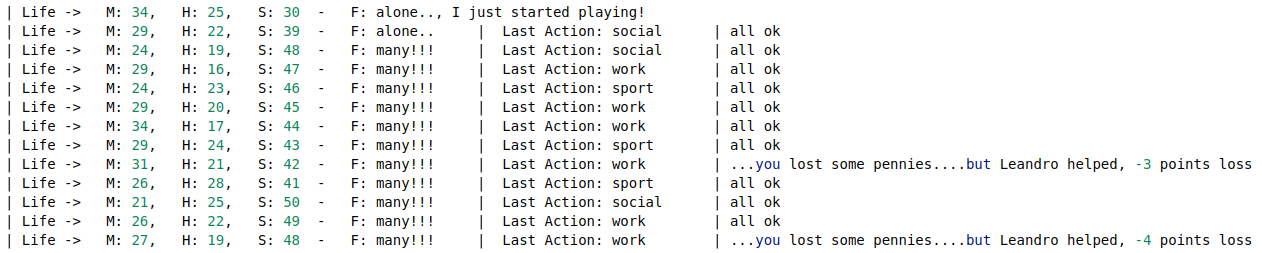
\includegraphics[width=0.95\linewidth]{img/example_A.png}
        \rule[-.5cm]{0cm}{0cm}}
  \caption{The start of an episode in monopoly mode}
  \label{fig:A}
\end{figure}

\section{Implementation}
This section will discuss the main parts related to the implementation of the architecture of the neural networks, the structure of the project files and the Jupyter Notebook.

\subsection{Project files}
The project is divided in multiple files. The \textit{agent.py and memory.py} files implement respectively the algorithm and the necessary memory structures. The notebook \textit{final.ipynb} uses the previous files to perform different training steps and showing the results.

The \textit{gym\_projects} directory contains everything related to the custom environment creation. The code of LifeSteps can be found in the \textit{lifesteps.py} file.

Since the notebook was executed three times with different seeds\footnote{\textit{final.ipynb} refers to the run with seed 14, and it's the only notebook with significant comments}, each run was saved into a different file. These files can be found in the \textit{notebook-runs} directory.

Tensorboard was used to log useful informations about the training. The logs directory is \textit{resources/logs/scalars}. Additionally, the outputs of the evaluations' prints of the notebooks were extracted into txt files inside the \textit{resources/logs/text} directory.

The \textit{models} directory contains the main checkpoints of the deep learning models.

\subsection{Notebook: final.ipynb}
The notebook has been executed three times, each one with a different seed. 
At the beginning of the notebook, the same seed for each run is set for the Numpy library, with the purpose of collecting a fixed list of evaluation seeds. As a result, the environments on which to perform the evaluation steps are the same for each run.
The notebook performs 4 main Steps:
\begin{itemize}
    \item Step 1: Training and evaluation in the standard game mode with a difficulty level of 40.
    \item Step 2: Fine-tuning and evaluation of the models from the previous step in the monopoly game mode with a difficulty level of 40.
    \item Step 3: Training and evaluation of new models, using the settings from Step 2.
    \item Step 4: Training and evaluation of new models with more units in the hidden layers, using the settings from Step 2.
\end{itemize}

The code was executed on a laptop with an Intel® Core™ i7-8565U CPU and an Nvidia MX250 2GB GPU.


\subsection{Deep learning architecture}
The Actor-Critic architecture was implemented using two separate neural networks (\(\rightarrow\) no weights sharing) with identical topology, except for the output layers. Each network consists of two hidden dense layer with 32 units each and hyperbolic tangent activations, followed by output heads with linear activations. In Step 4, the number of units was increased to 128 for both models. The notebook follows the fundamental characteristics of the original paper while incorporating some changes, which are described in comments.


\section{Results}
Table~\ref{results} summarizes the results of the evaluations for each step and seed, specifying some of the hyperparameters used.
The timesteps length of an episode was set to 100 and the difficulty level to 40. At each step, the training stopped after six consecutive evaluations that returned a cumulative reward higher than 0.

The number of Updates in the table refers to the lenght of the training at the time of the early stopping\footnote{Step 2 is the only one that starts from pre-trained neural networks, so even the number of updates of Step 1 should be considered.}.

\paragraph{A note on the evaluation values}
The values in the Evaluation column are the mathematical mean between the cumulative rewards of 50 episodes. The unbalanced nature of the rewards in LifeSteps should be taken into consideration when discussing the models' performances. 

\begin{table}
  \caption{Training results}
  \label{results}
  \centering
  \begin{tabular}{llcrcccc}
    \toprule
    Model & GM & Units & LR & \(c_2\) & Seed & Updates & Evaluation\\
    \midrule
    Step 1  & std & 32  & 2.5e-4  & 0 & 14 & 350 & \textbf{1.0} \\
    & & & & & 77 & 350 & 0.92 \\
    & & & & & 39 & 350 & 1.0 \\
    \midrule
    Step 2  & mon & 32  & 1e-4   & 5e-3 & 14 & 900 & -1.14\\
    & & & & & 77 & 2343 & -2.04 \\
    & & & & & 39 & 2343 & \textbf{0.66} \\
    \midrule
    Step 3  & mon & 32  & 2.5e-4  & 5e-3 & 14 & 2300 & \textbf{0.72}\\
    & & & & & 77 & 1150 & 0.66 \\
    & & & & & 39 & 3500 & 0.40 \\
    \midrule
    Step 4  & mon & 128 & 2.5e-4  & 5e-4 & 14 & 1750 & \textbf{0.86}\\
    & & & & & 77 & 2300 & 0.86 \\
    & & & & & 39 & 1250 & -0.96 \\
    \midrule
    random-bs  
            & std & & & & 14 & & -122.6 \\
    random-bs
            & mon & & & & 14 & & -123.4 \\
    
    \bottomrule
  \end{tabular}
\end{table}

\section{Discussion}

The PPO Agent solves easily the game in standard gamemode and difficulty 40, with only one lost game between the three runs. 

Step 2's goal was to understand if, starting from pre-trained networks, the training time to play a similar game could be reduced. The results suggest that fine-tuning the neural networks in this particular case does not result in a good evaluation score, most of the time.\footnote{even when fine-tuned models have a decent score, the training time is very long} 

This result isn't that much of a surprise. Since the state is encoded into a 4 values array of integers, the features that the networks need to learn are very simple. 
On the other hand, the policy to win a monopoly episode must be significantly different, and focus on boosting the sociality score from the start to reduce the penalties of chance cards.

Step 3 proves that the monopoly gamemode can be solved, even if the training time is longer than for the standard gamemode. The results are encouraging, the lost games usually where very near to be won by the agent. Another valuable information of this step is that a brand new untrained PPO Agent can perform better, with much less training, than a fine-tuned one taken from Step 2.

There is not a lot to say about Step 4, the results are positive but similar to Step 3, even with the significant increase in hidden layers' units.


\subsection{A deeper analysis}

During each evaluation step, some data about the model's behaviour was collected. To be more specific, it was considered useful to store the overall percentages of chosen actions. This data is described in Table~\ref{behaviour} and the values are taken from the best performer of each gamemode.

This data is much informative because it's not fine grained, but in a very simple way it describes the overall behaviour of the agent. In the monopoly gamemode, there is need of a more balanced policy for the selection of work and sport actions, to avoid losing the game. Sociality doesn't change much between the two gamemodes because the difficulty level is set to 40, which coincidentally is the threshold to get a new friend.

\begin{table}
  \caption{Agent's behaviour during the evaluation steps.}
  \label{behaviour}
  \centering
  \begin{tabular}{lcccc}
    \toprule
    gamemode & seed & work (\%) & sport (\%) & sociality (\%) \\
    \midrule
    standard & 14 & 54.8  & 32.8    & 12.4  \\
    monopoly & 14 & 53.4  & 34.5    & 12.0  \\
    \bottomrule
  \end{tabular}
\end{table}

A standard behaviour for the agent in monopoly mode is to improve the social score during the first timesteps, as seen in Figure~\ref{fig:A}. If this is not accomplished the game would be too hard to beat, as in Figure~\ref{fig:E}. In this example (step 4, seed 39, eval seed 40587), the agent fails to perform enough social actions in the first steps and acquire a friend, which would decrease the health and money losses after chance card events. Since the maximum deficit for a chance card while having a friend is 4, it's easy to see how, with social actions during the two first timesteps, the agent would have lost at least 18 points less. 

\begin{figure}
  \centering
  \fbox{\rule[-.5cm]{0cm}{0cm}
        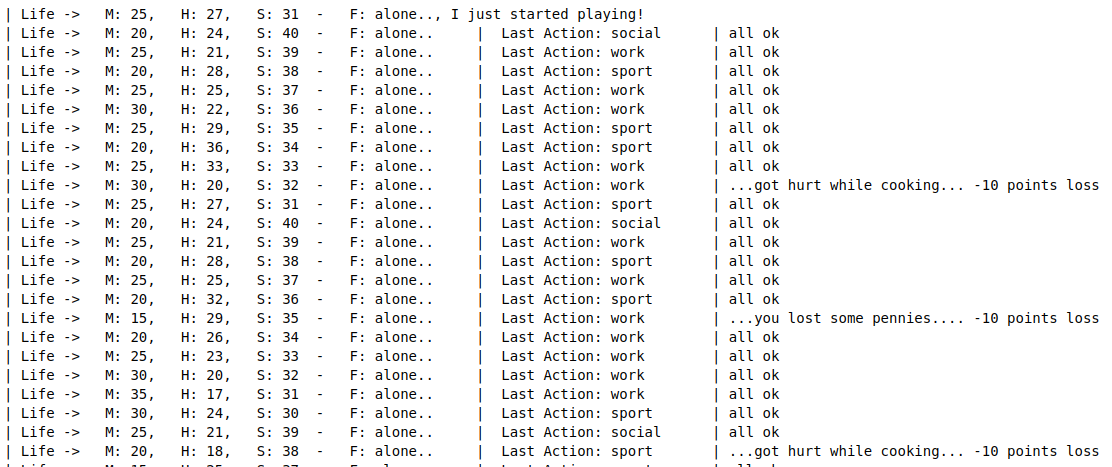
\includegraphics[width=0.95\linewidth]{img/example_E.png}
        \rule[-.5cm]{0cm}{0cm}}
  \caption{A failed monopoly game}
  \label{fig:E}
\end{figure} 

Additionaly, the policy does something strange at the end of a monopoly episode. As can be seen in Figure~\ref{fig:F} (step 4, seed 39, eval seed 75763), the player has a very high social score at the end of the simulation. The actual social score needed to win the game (in that difficulty level) was 40. On the contrary, the money score is 43, so it seems like the agent takes an unnecessary risk on developing sociality more than it's actually needed.

\begin{figure}
  \centering
  \fbox{\rule[-.5cm]{0cm}{0cm}
        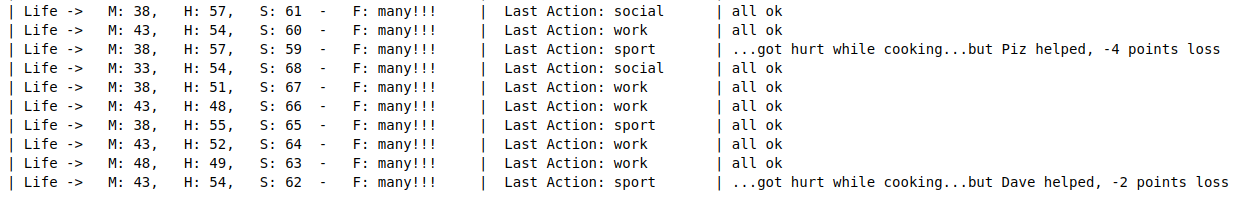
\includegraphics[width=0.95\linewidth]{img/example_F.png}
        \rule[-.5cm]{0cm}{0cm}}
  \caption{Unbalanced life scores at the end of a monopoly episode}
  \label{fig:F}
\end{figure}

A more robust behaviour can be observed at the end of a standard episode, which at the end of the game results in a more balanced life score. 

To understand more the behaviour of the agents it's advisable to read the text logs of the evaluations.

The Tensorboard logs will not be exposed in the report because, even if useful to find problems during the design and programming of the project, they don't give out much useful informations at the end.

% % % % % % % % % % % % % % % % % % % % % % % % % % % % %
% % % % % % % % % % % % % % % % % % % % % % % % % % % % %
\section{Conclusions}

The LifeSteps environment works correctly and the implemented agent is able to solve the game without many errors. When the game gets difficult, e.g. in monopoly episodes, the agent can still win games, but the behaviour seems to be risky and the strategy isn't optimal. Obviously the agents could've been trained more and maybe reach perfect scores even in monopoly gamemode, but that level of performance was not the goal of the project. 

Using vectors of environments proved to be very useful to shorten the length of the training, along with the possibility to run many parallel \textit{notebooks}. The agents for the monopoly gamemode would have been very hard to train with a single environment. 

The agent was used (with very little code tweaks) with other environments (e.g. CartPole) to be sure that the algorithm worked well even in different conditions. 

The performance of the trained models seem to be dependend on the seed. This may be for many reasons such as the randomness and difficulty of the game, or the lack of enough exploration to avoid getting stuck in a local minimum. An exhaustive search of optimal hyperparameters (e.g. the entropy bonus) may lead to better performance.


\section{Useful links}
Project code: \href{https://github.com/ancaah/autonomous}{github.com}

The following arcticles were read during the debug process.

\textit{The 37 implementation details of PPO} was an interesting read to understand details about why to use certain activations, weights network initialization, advantages and returns normalization: \href{https://iclr-blog-track.github.io/2022/03/25/ppo-implementation-details/}{iclr-blog-track.github.io}

The \textit{CleanRL PPO implementation} was useful for checking the correctness of my code: \href{https://github.com/vwxyzjn/cleanrl/blob/master/cleanrl/ppo.py}{github.com}

This repository suggested the idea of dividing the code into more files, simplifying the debug and test activities: \href{https://github.com/philtabor/Youtube-Code-Repository/blob/master/ReinforcementLearning/PolicyGradient/PPO/tf2/memory.py}{github.com}

The report was written in english using Overleaf (\href{http://overleaf.com}{overleaf.com}) and the phrasing corrected using ChatGPT (\href{https://chat.openai.com}{openai.com})
%%%%%%%%%%%%%%%%%%%%%%%%%%%%%%%%%%%%%%%%%%%%%%%%%%%%%%%%%%%%

\bibliography{citations}

\end{document}